\documentclass[a4paper,11pt]{article}
%\usepackage{array}
%\usepackage{theorem}
\usepackage{graphicx}
\usepackage{fancyhdr}
%\usepackage{times,mathptm}
%\usepackage[pdftex]{graphicx}
%\usepackage{color}
%\usepackage{caption}
%\usepackage{graphpap}
%\usepackage{rotating}
%\usepackage{epsfig}
%\usepackage{epsfig,psfrag}

%\setlength{\textwidth}{6.0in}
%\setlength{\textheight}{8.0in}
%\setlength{\topmargin}{0.in}
%\setlength{\headheight}{0.8in}
%\setlength{\headsep}{0.in}
%\setlength{\parindent}{0.25in}
%\setlength{\oddsidemargin}{0.2in}
%\setlength{\evensidemargin}{0.2in}

\newcommand{\ve}[1]{\mbox{\boldmath $ #1$}}
%opening
\title{TDStool: Notes on Numerical Methods}
\author{Andrea Bertoni, Thomas Serafini}



\begin{document}

%\setlength{\leftmargini}{\parindent} % Controls the indenting of the "bullets" in a list
%\pagestyle{empty}
%\pagenumbering{alph}
%\begin{minipage}[t][7.5in][s]{6.25in}
\begin{titlepage}

\flushright{
\Huge
TDS{\hspace{1mm}}tool}

\flushright{
\LARGE
\mbox{Time Dependent Schr{\"o}dinger equation simulation tool}}

\vspace{40mm}
\flushright{
\huge
\bf Notes on Numerical Methods}

\vspace{20mm}
\flushright{
\Large
Andrea Bertoni \\
\vspace{2mm}
Thomas Serafini}

\vspace{60mm}
\flushright{
\large
\today \\
Version 0.2 \\
TDStool Version 0.2}

\vspace{10mm}
\flushright{
\Large
S3 National Research Center, CNR-INFM \\ Modena, Italy}

\normalsize
%\vfill
% \flushright{\includegraphics[width=2.in]{FIGURES/nistident_flright_vec}}

\newpage
\pagestyle{empty}
\mbox{}
\end{titlepage}
%\end{minipage}
%\maketitle
%\begin{abstract}
%\end{abstract}

\section*{Preface}
The software TDStool is a numerical solver for the Time Dependent (linear)
Schr\"odinger equation and (nonlinear) Gross-Pitaevskii equation.
This document provides the theoretical basis for TDStool.
It describes the discretization methods and the main numerical
algorithms used in the code. It aims to be a technical reference guide
and a means to reach an in-depth understanding of the source code.
In fact, it should be the starting point for whoever is willing to
modify the code (released as an open-source project) and hopefully contribute
to the project.
Since the discussion in this note has been kept at a tutorial level, 
it can represent a nimble introduction to some of the numerical techniques
used in the code. However, we urge any 


\section*{Disclaimer}
We make no warranty to users of TDStool and accept no responsability for
its use and for any conclusion drawn from its results.  Although we endeavor
to 


TDStool is intended
for use only by those competent in the field of quantum mechnaics and
numerical analysis.

\section*{Copyright}
ccc

\section*{About the Authors}
(up-to-date as of \today)

{\bf Andrea Bertoni} is

{\bf Thomas Serafini} is

\section*{Acknowledgments}
zzz

\newpage

\tableofcontents

\newpage

\pagestyle{fancy}
\fancyhead[RO,RE]{TDStool: Notes on Numerical Methods}
\fancyhead[LO,LE]{ver. 0.2}

\section{Notation}
Let $f$ be a functional $f:R^n\mapsto C$.
$$ F = \bigtriangledown f = \mbox{grad}(f) = (F_1, \cdots, F_n) =
  \left( \frac{\partial f}{\partial x_1}, \cdots, \frac{\partial f}{\partial x_n} \right) $$
$$ div(F) = \bigtriangledown \cdot F = \frac{\partial F}{\partial x_1} + \cdots + \frac{\partial F}{\partial x_n} $$
$$ \bigtriangledown^2 f = \bigtriangledown \cdot \bigtriangledown f =
    \frac{\partial^2 f}{\partial x_1^2} + \cdots + \frac{\partial^2 f}{\partial x_n^2} $$

\section{Scr\"{o}dinger equation}
We want to solve the time-dependent Scr\"{o}dinger equation on a domain with Dirichlet boundary conditons, starting from the wave function $\psi(0)$ at the initial time. The equation is:
$$ i \hbar \frac{\partial}{\partial t} \psi(t) = H \psi(t) $$
where $ H = - \frac{\hbar^2}{2m^*}\partial_x^2 + V(x) $.
The equation can be rewritten as:
\begin{eqnarray}
\frac{\partial \psi}{\partial t} & = & \beta \bigtriangledown G + v\psi \\
G & = & \bigtriangledown \psi
\end{eqnarray}
$$ \psi \in D, \quad \psi = g \ \mbox{on} \ \partial D $$
where $\beta = - \frac{1}{i \hbar} \frac{\hbar^2}{nm^*} = i \frac{\hbar}{2m^*} $
and $ v = \frac{1}{i \hbar} V = -\frac{i}{\hbar}V $

\section{Box Integration Method}
We start by semidiscretizing the Scr\"{o}dinger equation in the space. We work on a special case where the domain is a box and the dicretization grid is orthogonal and separable. For simplicity we are going to consider a 2D grid, but the discretization can easily be extedned to a higher dimensional domain.

Let $D = [x_0, x_{n+1}] \times [y_0, y_{m+1}]$ be a quare domain.
Let $ x_0 < x_1 < \cdots < x_{n+1} $ and $ y_0 < y_1 < \cdots < y_{m+1} $ be the coordinates of an orthogonal grid. We will have $nm$ internal nodes in which the function $\psi$ is unknown. The function $\psi(x, y, t)$ in the points where $x = x_0$ or $x = x_{n+1}$ or $y = y_0$ or $y = y_{m+1}$ is known thanks to the Dirichlet boundary contitions.
We consider a vertex-centered Box Integration Method: this means that we divide the domain $D$ into $nm$ boxes $C_{ij} = [\frac{x_i - x_{i-1}}{2}, \frac{y_i - y_{i-1}}{2}] \times
                [\frac{x_{i+1} - x_i}{2}, \frac{y_{i+1} - y_i}{2}] $.
If we call $a_i = x_i - x_{i-1}, \quad i = 1, \cdots, n+1$ and
$b_j = y_j - y_{j-1}, \quad j = 1, \cdots, m+1$, a box $C_{ij}$ has area
$s_{ij} = \frac{a_i+a_{i+1}}{2} \frac{b_i+b_{i+1}}{2}$.
In the Box Integration Method we integrate the equation on each box $C_{ij}$:
$$ \int_{C_{ij}} \frac{\partial \psi}{\partial t} ds = 
   \beta \int_{C_{ij}} \bigtriangledown G ds + 
   \int_{C_{ij}} v \psi ds $$

The three integrals can be approximated as follow:
\begin{eqnarray}
\int_{C_{ij}} \frac{\partial \psi}{\partial t} ds & \approx &
   s_{ij} \frac{d \psi}{dt}(x_i, y_j, t) \\
\int_{C_{ij}} v \psi ds & \approx & s_{ij} (v \psi)(x_i, y_j, t) \\
\int_{C_{ij}} \bigtriangledown G ds = \oint_{\partial C_{ij}} G \bar{\ve{n}} dl & \approx &
   (G_e \bar{\ve n}_e + G_n \bar{\ve n}_n + G_w \bar{\ve n}_w + G_s \bar{\ve n}_s) \label{green_int}
\end{eqnarray}

where $\bar{\ve n}_e, \bar{\ve n}_n, \bar{\ve n}_w, \bar{\ve n}_s$ are the vectors normal to the four edges of the box, whose modulus is equal to the lenght of the edge (area of the surface in the 3D case), and $G_e, G_n, G_w, G_s$ are gradients in the mid point of each edge, as shown in Figure.

\begin{figure}
 \label{fig:single_box}
\centerline{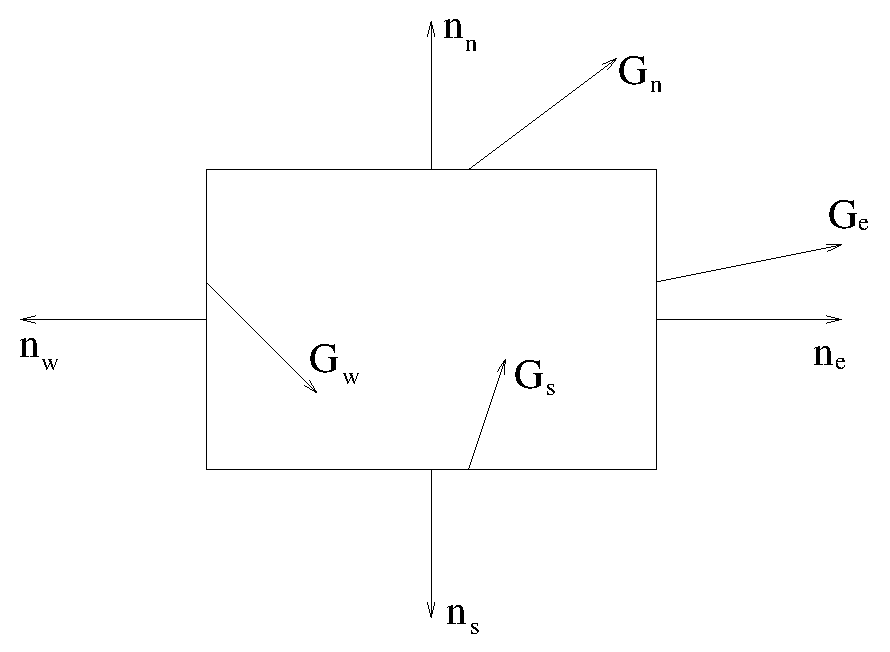
\includegraphics[width=2in] {box.eps}}
\caption{Single box scheme}
\end{figure}

Let $y \in R^{nm}$ be the space-discretized wave function: $y_{ij}(t) = \psi(x_i, y_i, t)$. For ease of notation, we sometimes repreent an element of $y$ with a double index ($y_{ij}$): this implicitly means that we are accessing the element $y_{im+j}$, i.e. the vector $y$ is a column-wise representation of the space-dicretization of $\psi$.
Usign a centered difference formula, the gradient values can be aproximated from the $y$ values on the nodes and the approximation of integral \ref{green_int} becomes:
$$ \frac{y_{i,j}-y_{i-1,j}}{a_i} \frac{b_j+b_{j+1}}{2} +
   \frac{y_{i,j}-y_{i+1,j}}{a_{i+1}} \frac{b_j+b_{j+1}}{2} +
   \frac{y_{i,j}-y_{i,j-1}}{b_j} \frac{a_i+a_{i+1}}{2} +
   \frac{y_{i,j}-y_{i,j+1}}{b_{j+1}} \frac{a_i+a_{i+1}}{2} $$

Let define
$$ k_1 = \frac{b_j+b_{j+1}}{2a_i}, \qquad k_2 = \frac{b_j+b_{j+1}}{2a_{i+1}} $$
$$ k_3 = \frac{a_i+a_{i+1}}{2b_j}, \qquad k_4 = \frac{a_i+a_{i+1}}{2b_{j+1}} $$

The approximation of integral \ref{green_int} becomes:
$$ (k_1+k_2+k_3+k_4) y_{i, j} + k_1 y_{i-1,j} + k_2 y_{i+1,j} + k_3 y_{i,j-1} + k_4 y_{i,j+1} $$
If a box is on the boundary of the domain, some of the $y$ terms of the summation are defined by the boundary conditions rather than being unknown. In this case we can group all these terms in one constant term. For example, if $(i, j) = (1, 1)$, then $y_{i-1,j}$ and $y_{i,j-1}$ are on the boundaries and the above expression becomes
$$ (k_1+k_2+k_3+k_4) y_{i, j} + k_2 y_{i+1,j} + k_4 y_{i,j+1} + d_{ij}$$
with $ d_{ij} = k_1 y_{i-1,j} + k_3 y_{i,j-1} $.

In vector form, these summations can be represented as a scalar product $\ve m_{ij} y + d_{ij}$ with $\ve m_{ij} \in R^{nm}$ and
$\ve m_{ij} = (0,\cdots, 0, k_1, 0, \cdots, 0, k_3, k_1+k_2+k_3+k_4, k_4, 0,\cdots, 0, k_2, 0, \cdots, 0)$.

Thus, the Scr\"{o}dinger equation can be approximately integrated on the box $C_{ij}$ with
$$ s_{ij} \frac{d y_{ij}}{dt}(t) =  \beta \ve m_{ij} y(t) + s_{ij} v_{ij} y_{ij}(t) + \beta d_{ij}$$

Let $S = \mbox{diag}(s_{ij})$ and $M = \beta [\ve m_{ij}] + \mbox{diag}(s_{ij}v_{ij})$: the equation can be written in matrix form:
$$ S \frac{d \ve y}{dt}(t) = M \ve y(t) + \beta \ve d$$

The time discretization of the above equation with the trapezoidal rule becomes:
$$ S \ve y^{(n+1)} = S \ve y^{(n)} + \frac{M \Delta t}{2} (\ve y^{(n)} + \ve y^{(n+1)}) + \beta \Delta t \ve d$$
or equivalently
$$ \left( S - \frac{M \Delta t}{2} \right) \ve y^{(n+1)} = \left( S + \frac{M \Delta t}{2} \right) y^{(n)} + \beta \Delta t \ve d $$

\end{document}
